\documentclass{beamer}
\usepackage{amsmath}
\usepackage{amssymb}
\usepackage{physics}
\usepackage{amsthm}
\usepackage{graphicx}
\usepackage{caption}
\usepackage{subcaption}
\usepackage{listings}
\graphicspath{ {./figures/} }
\title{Aplikace spektrální metody}
\author{Dominika Hájková, Matyáš Fuksa, Ondřej Kureš}
\institute{Stormtrooperz}
\date{2021}

\begin{document}


\frame{\titlepage}
\begin{frame}
\frametitle{Spektrální metoda - Co to je?}
Povíme něco o spektrální metodě jako takové.
\end{frame}

\begin{frame}[fragile]
\frametitle{Trám na jiný způsob - Kód}
\begin{lstlisting}[language=Matlab, basicstyle=\small, numbers=left,breaklines=true]
f = @(x) 75*9.81*exp(-x.^2/(2*0.01)); alpha = 0; beta = 0; gama = 0 ;delta = 0; n = 18; E = 9.4*10^6; Izz = 3;l = 10;X = [-l/2,l/2];
L = E*Izz*diffmat([n n+4],4,X);
vT = diffrow(n+4,0,-l/2,X); wT = diffrow(n+4,0,l/2,X); uT = diffrow(n+4,1,-l/2,X); sT = diffrow(n+4,1,l/2,X);
A = [L; vT; wT; uT; sT];
rhs = [gridsample(f,n); alpha; beta; gama; delta];
u = A\rhs;
tiledlayout(2,1)
nexttile
plot(chebfun(-u,X),'.-');ylim([-1 1]);
nexttile
plot(chebfun(-u,X),'.-');ylim([-0.001 0.001])
\end{lstlisting}
\end{frame}

\begin{frame}
\frametitle{Trám na jiný způsob - Obrázky}
\centering
\begin{figure}
\includegraphics[width=.9\linewidth]{První.png}
\includegraphics[width=.9\linewidth]{Druhý.png}
\caption{Musím doplnit}
\end{figure}
\end{frame}

\begin{frame}
\frametitle{Kmitání membrán - Analytický rozbor}
\begin{equation}
\Delta u=-\lambda u
\end{equation}
\begin{equation}
u(x,y)=X(x) Y(y)
\end{equation}
\begin{equation}
   \frac{\partial^2 X}{\partial x^2} Y
      + X \frac{\partial^2 Y}{\partial y^2}=-\lambda X Y
\end{equation}
\begin{equation}
X(0)=X(a)=0
\end{equation}
\begin{equation}
Y(0)=Y(b)=0
\end{equation}
\begin{equation}
X(x)=A_1 \sin{(\sqrt{\lambda-\alpha}x)}+B_1 \cos{(\sqrt{\lambda-\alpha}x)}
\end{equation}
\begin{equation}
Y(y)=A_2 \sin{(\sqrt{\alpha}y)}+B_2 \cos{(\sqrt{\alpha}y)}
\end{equation}
\begin{equation}
\lambda_{m,n}=\frac{m^2\pi^2}{a^2}+\frac{n^2\pi^2}{b^2}
\end{equation}
\begin{equation}
u(x,y)_{m,n}=A\sin{(\frac{m\pi}{a}x)}\sin{(\frac{n\pi}{b}y)}
\end{equation}
\end{frame}

\begin{frame}
\frametitle{Kmitání membrán - Analytický rozbor}
\end{frame}

\begin{frame}
\frametitle{Kmitání membrán - Numerické řešení}
\end{frame}

\begin{frame}
\frametitle{Kmitání membrán - Výsledky 1. část}
\centering
\begin{figure}
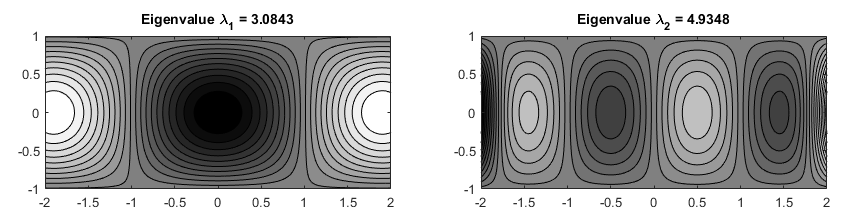
\includegraphics[width=1\linewidth]{obdelnicky1.png}
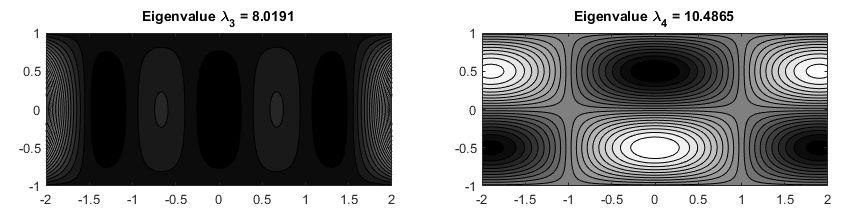
\includegraphics[width=1\linewidth]{obdelnicky2.png}
\caption{Získáno v Matlabu}
\end{figure}
\end{frame}

\begin{frame}
\frametitle{Kmitání membrán - Výsledky 2. část}
\centering
\begin{figure}
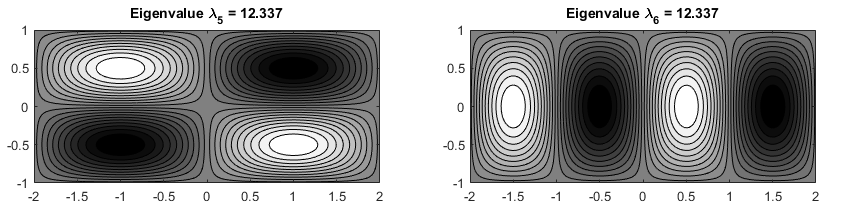
\includegraphics[width=1\linewidth]{obdelnicky3.png}
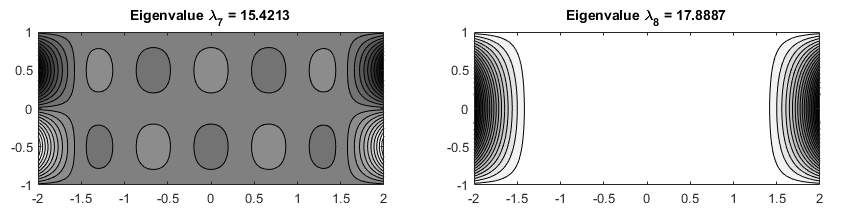
\includegraphics[width=1\linewidth]{obdelnicky4.png}
\caption{Získáno v Matlabu}
\end{figure}
\end{frame}

\begin{frame}
\frametitle{Kmitání membrán - Výsledky 3. část}
\centering
\begin{figure}
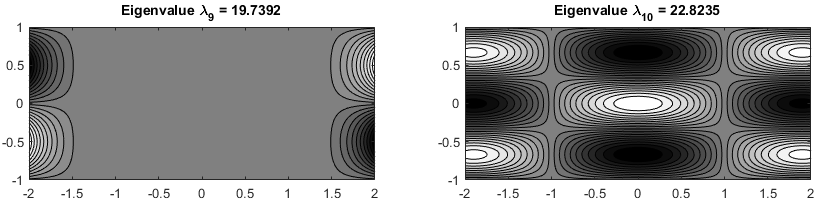
\includegraphics[width=1\linewidth]{obdelnicky5.png}
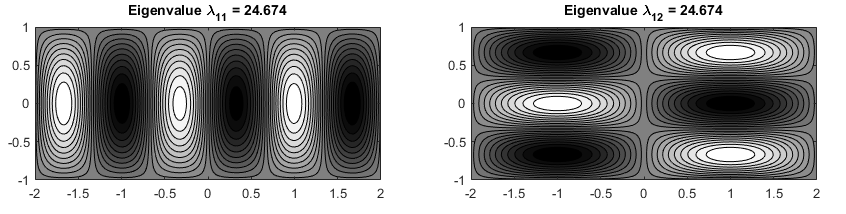
\includegraphics[width=1\linewidth]{obdelnicky6.png}
\caption{Získáno v Matlabu}
\end{figure}
\end{frame}

\begin{frame}
\frametitle{Kmitání membrán - Výsledky 4. část}
\centering
\begin{figure}
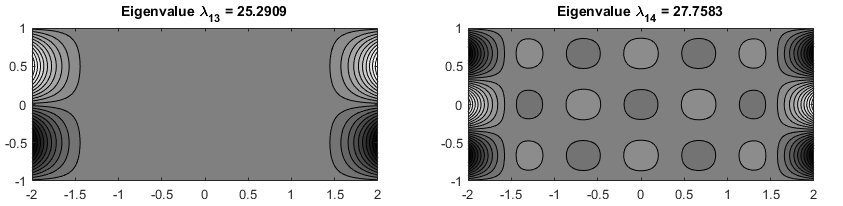
\includegraphics[width=1\linewidth]{obdelnicky7.png}
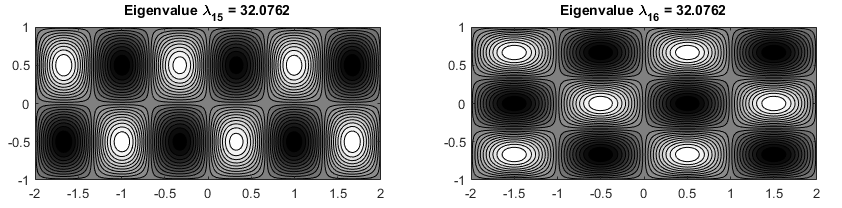
\includegraphics[width=1\linewidth]{obdelnicky8.png}
\caption{Získáno v Matlabu}
\end{figure}
\end{frame}

\begin{frame}
\frametitle{Kmitání membrán - Výsledky 5. část}
\centering
\begin{figure}
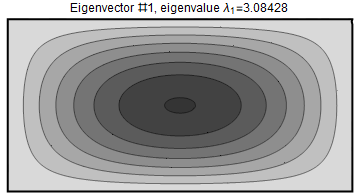
\includegraphics[width=.6\linewidth]{rectangle-eigenvector-1.png}
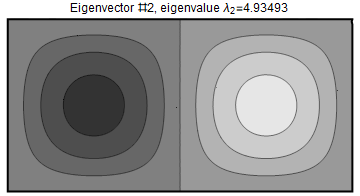
\includegraphics[width=.6\linewidth]{rectangle-eigenvector-2.png}
\caption{Získáno v Mathematice}
\end{figure}
\end{frame}

\begin{frame}
\frametitle{Kmitání membrán - Výsledky 6. část}
\centering
\begin{figure}
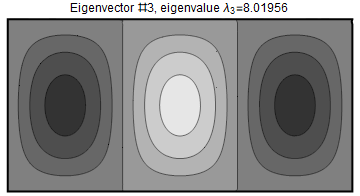
\includegraphics[width=.6\linewidth]{rectangle-eigenvector-3.png}
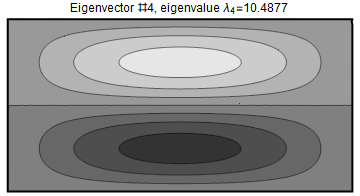
\includegraphics[width=.6\linewidth]{rectangle-eigenvector-4.png}
\caption{Získáno v Mathematice}
\end{figure}
\end{frame}

\begin{frame}
\frametitle{Kmitání membrán - Výsledky 5. část}
\centering
\begin{figure}
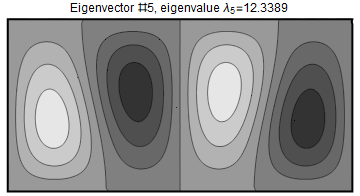
\includegraphics[width=.6\linewidth]{rectangle-eigenvector-5.png}
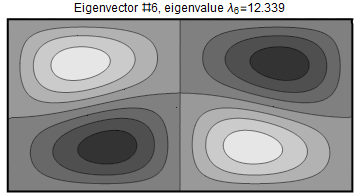
\includegraphics[width=.6\linewidth]{rectangle-eigenvector-6.png}
\caption{Získáno v Mathematice}
\end{figure}
\end{frame}

\begin{frame}
\begin{center}
\begin{huge}
Děkujeme za pozornost
\end{huge}
  \centering
  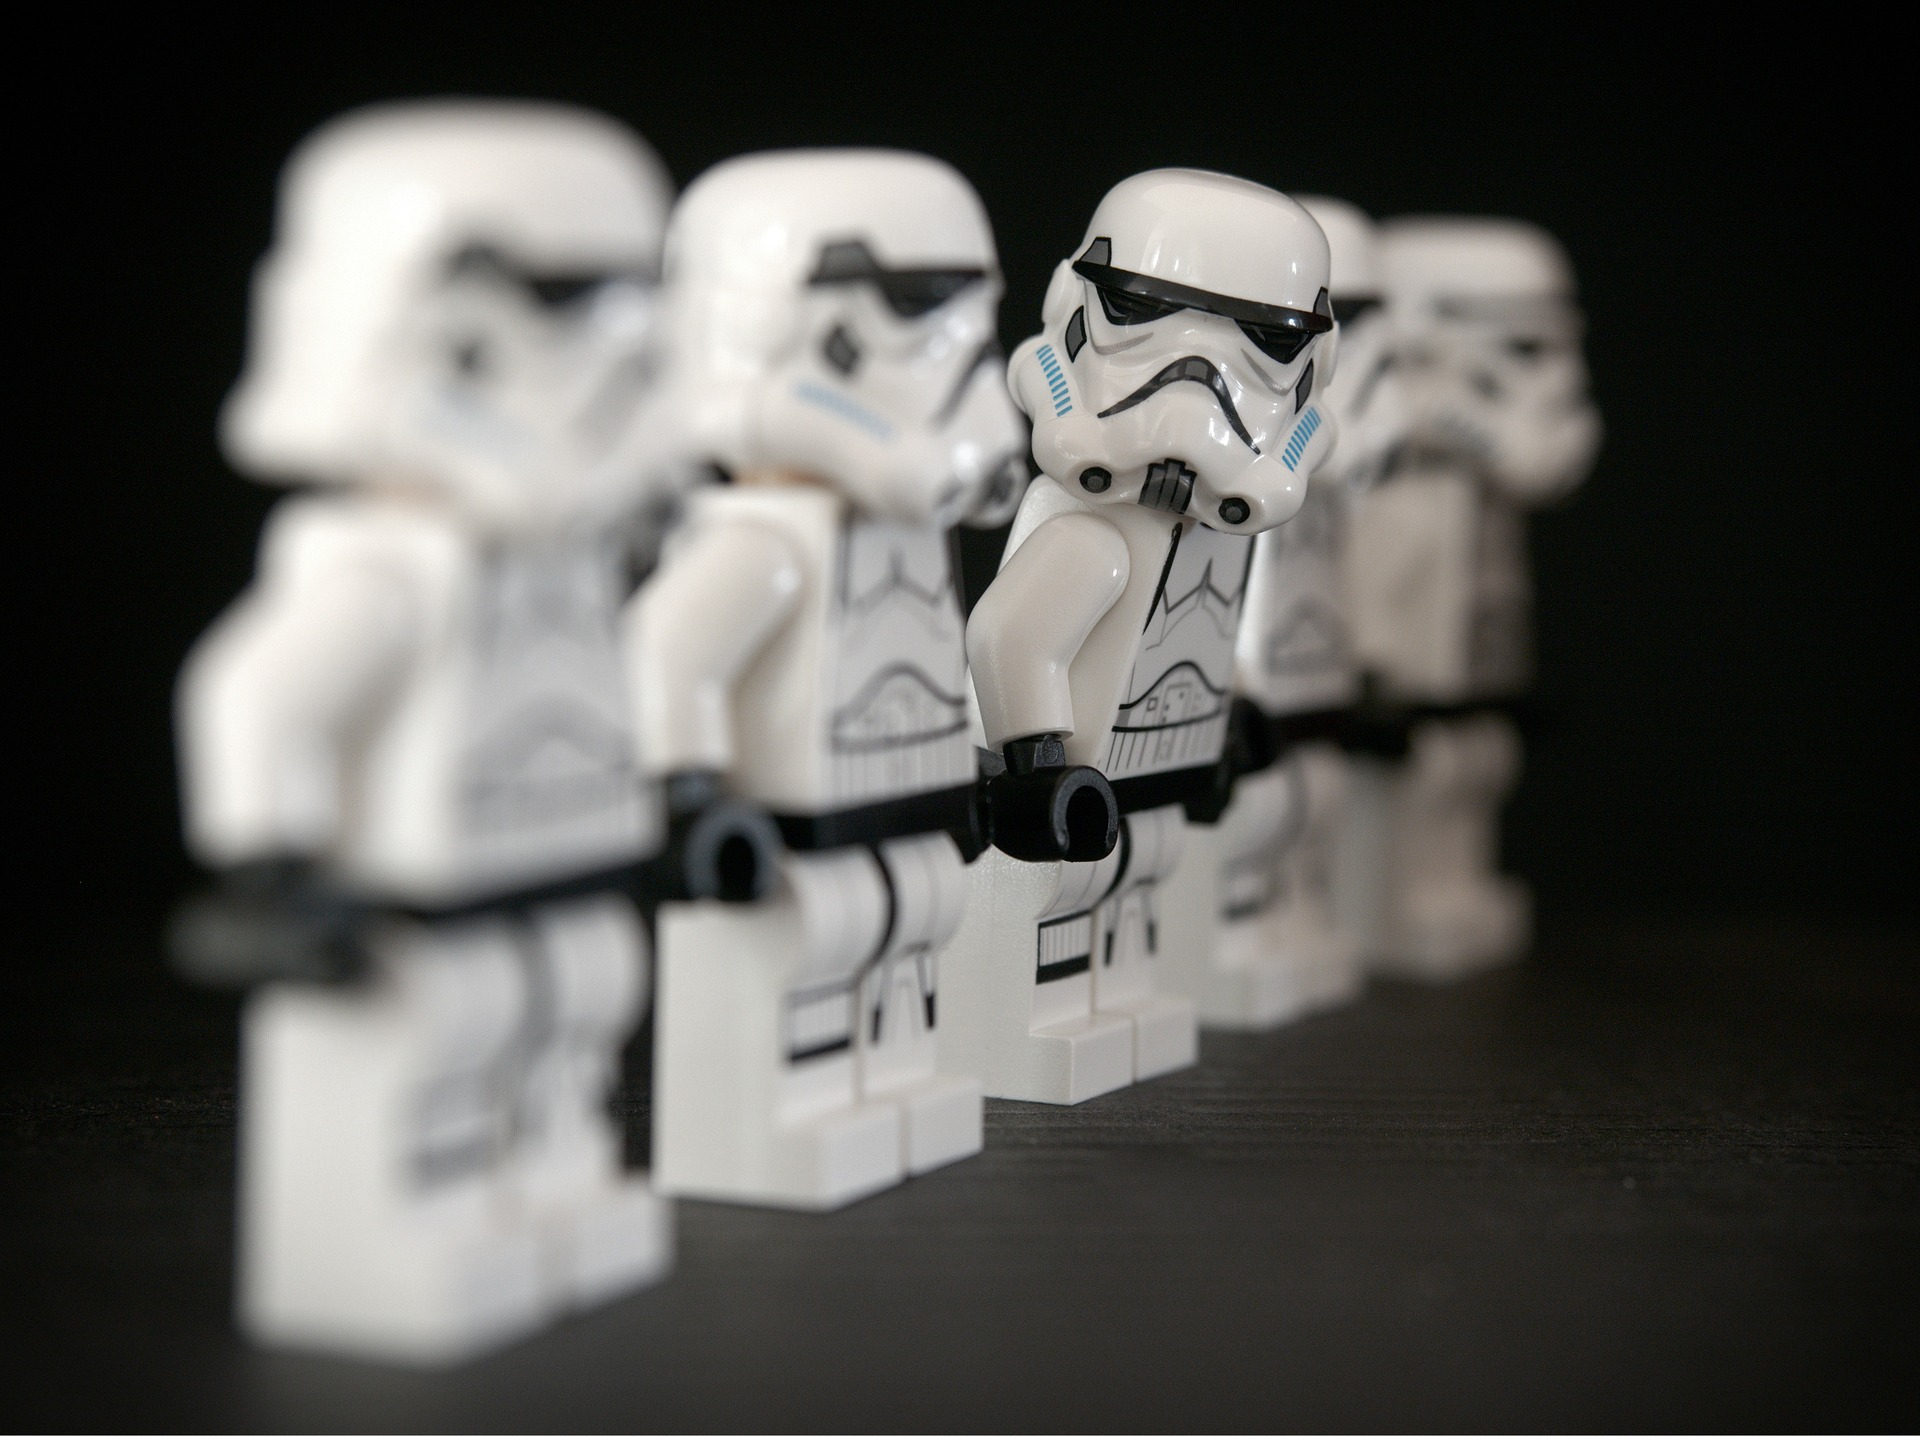
\includegraphics[width=.8\linewidth]{stormtroop.jpg}
\end{center}

\end{frame}
\end{document}